\documentclass[article,36pt,extrafontsizes,oneside,openany,oldfontcommands]{memoir}
\usepackage{graphicx}
    \graphicspath{{figure/}}
\usepackage{amsmath, amsfonts, amssymb, amsthm}
\usepackage{mathtools}
\usepackage[charter,expert]{mathdesign}
\usepackage{fontspec}
\usepackage{xltxtra, xunicode}
\usepackage[utf8]{inputenc}
\RequirePackage[CJKmath = true, 
                indentfirst = false, 
                PunctStyle = {quanjiao}, 
                CheckSingle = true, 
                SlantFont, 
                BoldFont]
                {xeCJK}
%\usepackage{lmodern}
%\usepackage{times}
%\usepackage{mathptmx}
%\usepackage[minionint, lf, mathtabular]{MinionPro}
\usepackage{bm}
\RequirePackage{lipsum}
\RequirePackage{blindtext}
\RequirePackage[svgnames,table]{xcolor}
\RequirePackage{tikz}
\RequirePackage[framemethod=tikz]{mdframed}
\RequirePackage{color}
\RequirePackage{geometry}
\RequirePackage{adjmulticol}
\RequirePackage[skins,most,listings,skins]{tcolorbox}

%For kable extra package :)
\RequirePackage{longtable}
\RequirePackage{array}
\RequirePackage{multirow}
\RequirePackage{wrapfig}
\RequirePackage{float}
\RequirePackage{colortbl}
\RequirePackage{pdflscape}
\RequirePackage{pagecolor}
\RequirePackage{tabu}
\RequirePackage{threeparttablex}
\RequirePackage[normalem]{ulem}
\RequirePackage{makecell}
\RequirePackage{wrapfig}
\usepackage{xmpmulti, booktabs, multicol}
\usepackage{threeparttable}
\usepackage{dcolumn}
\newcolumntype{.}[1]{D{.}{.}{#1}}
\newcolumntype{,}[1]{D{,}{,}{#1}}
\usepackage{siunitx}
\sisetup{%
  mode = math,
  detect-all,  
  output-decimal-marker = {.},
  group-separator = {,},
  math-rm = \rmnumeric,
  text-rm = \rmnumeric,
}

%rof hyperrefs
\usepackage{color}
    \definecolor{MyBrown}{HTML}{3D3D00}
    \definecolor{MyBlue}{HTML}{003A75}  
    \definecolor{MyRed}{HTML}{6F1A2F}
    \definecolor{MyGreen}{HTML}{004847}
\usepackage{hyperref}
    \hypersetup{bookmarks = true,
                bookmarksnumbered = true,
                colorlinks = true,
                linkcolor = MyRed,
                citecolor = MyBlue, % hyperref is in conflict with natbib
                filecolor = MyBrown,
                urlcolor = MyGreen}
%For figure and table placement
\RequirePackage{float}
\floatplacement{figure}{H}
\floatplacement{table}{H}

%%%%%%%%% COLOURS %%%%%%%%
%Fill/ Line Colours
\definecolor{titleboxbgcol}{HTML}{D8E0FF}
\definecolor{titleboxbordercol}{HTML}{205DA4}
\definecolor{columnlinecol}{HTML}{008080}
\definecolor{bodybgcol}{HTML}{ffffff}
\definecolor{sectitlebgcol}{HTML}{D8E0FF}
\definecolor{sectitlebordercol}{HTML}{D8E0FF}
% Text Colours
\definecolor{titletextcol}{HTML}{1c518f}
\definecolor{authortextcol}{HTML}{000000}
\definecolor{affiliationtextcol}{HTML}{000000}
\definecolor{sectitletextcol}{HTML}{1c518f}
\definecolor{bodytextcol}{HTML}{000000}
\definecolor{footnotetextcol}{HTML}{000000}
\definecolor{citecol}{HTML}{CC0000}
\definecolor{urlcol}{HTML}{008080}
\definecolor{linkcol}{HTML}{008080}


%Memoir spacing options
%spacing between figure/ table and caption
\setlength{\abovecaptionskip}{0.4in}
\setlength{\belowcaptionskip}{0.2in}
\captionnamefont{\large}
\captiontitlefont{\large}

%define column options
\setlength{\columnseprule}{0pt}
\def\columnseprulecolor{\color{columnlinecol}}

%define section title features
\setsubsubsecheadstyle{\small\color{sectitletextcol}\textbf}% Set \section style
\setsecnumformat{}
\def\sectionmark#1{\markboth{#1}{#1}}

%%%%%%%%%%%% TCOLORBOXES TO THE RESCUE %%%%%%%%%%%%%%%%%%%%
%Title Box
\newtcolorbox{topbox}{
enhanced,
colback=titleboxbgcol,
colframe=titleboxbordercol,
halign=center,
boxrule=0cm,
sharp corners=all,
 overlay={
    % \node[anchor=south west]
    %   at ([xshift=1in,yshift=1in]frame.south west)
    %    {\includegraphics[width=3in]{Figures/posterdownlogo}};
    % \node[anchor=south east]
    %   at ([xshift=-1in,yshift=1in]frame.south east)
    %    {\includegraphics[width=3in]{Figures/posterdownlogo}};
       }

}
%Body Section Title Box
\newtcolorbox{myboxstuff}[1][]{
code={\parindent=0em},
colframe=sectitlebordercol,
nobeforeafter,
left skip=0pt,
valign=center,
halign=center,
fontupper=\Large\bfseries,
colupper=sectitletextcol,
boxrule=2mm,
colback=sectitlebgcol,
sharp corners=south, #1}
\newcommand{\mybox}[1]{%
\begin{myboxstuff}
\strut #1
\end{myboxstuff}%
}
\makeheadstyles{MyBox}{
    \setsecheadstyle{\mybox}
}
\headstyles{MyBox}\makepagestyle{MyBox}
%-----------------------------------------------------
%Make sure that the page is empty of any preset items from memoir
\thispagestyle{empty}

%biblatex options
%\usepackage{natbib}
%\DeclareTextCommandDefault{\nobreakspace}{\leavevmode\nobreak\ } % AER style nobreak
\renewcommand{\bibname}{\hrule}
%\renewcommand{\bibsection}{}
%\renewcommand*{\bibfont}{\fontsize{40pt}{45pt}\selectfont}
%\setlength{\bibsep}{0pt plus 0.3ex}

%Remove section numbering & set 2nd level header as first level
%to avoid the automatic new page generated from memoir chapter
%formatting
\counterwithout{section}{chapter}
\makechapterstyle{mydefault}{
\addtocounter{secnumdepth}{2}
\setsecheadstyle{\mybox}
\setsubsecheadstyle{\itshape}
\setsubsubsecheadstyle{\itshape}
}

%set the chapterstyle
\chapterstyle{mydefault}

%define column spacing
\setlength\columnsep{0.5in}

%spacing params
\setlength\parindent{0em}
\setlength\parskip{0em}
\setlength\hangparas{0em}

%spacing after section head title
\setaftersecskip{0em}
\setbeforesecskip{1.5em}
\setlength\textfloatsep{0in} % distance between floats on the top or the bottom and the text
\setlength\floatsep{0.1in} % distance between two floats
\setlength\intextsep{0.5in} % distance between floats inserted inside the page text (using h) and the text proper
\makeatletter
\g@addto@macro{\normalsize}{%
%    \setlength\abovedisplayskip{30pt} % spacing above equations
%    \setlength\abovedisplayshortskip{15pt} % spacing immediately above equations
%    \setlength\belowdisplayskip{0pt} % spacing below equations
%    \setlength\belowdisplayshortskip{0pt} % spacing immediately below equations
%    \setlength{\displayindent}{0in}
%    \setlength{\predisplaysize}{0in}
    } 
\makeatother

\setstocksize{36in}{48in}
\settrimmedsize{\stockheight}{\stockwidth}{*}
\settypeblocksize{36in}{48in}{*}
\setlrmargins{*}{*}{1}
\setulmarginsandblock{2.5cm}{0cm}{*}
\setmarginnotes{0em}{0cm}{0cm}
\setlength{\footskip}{0cm}
\setlength{\footnotesep}{0cm}
\setlength{\headheight}{0pt}
\setlength{\headsep}{0pt}
\setlength{\trimtop}{0pt}
\setlength{\trimedge}{0pt}
\setlength{\uppermargin}{0pt}
\checkandfixthelayout
\usepackage{enumitem}
\usepackage{bbm}
\usepackage{dsfont}
\def\one{\mathrm{1}\hspace{-12pt}\mathrm{1}}
\setlist[enumerate]{topsep=0pt,itemsep=-1ex,partopsep=1ex,parsep=1ex,leftmargin=2ex}
\setlist[itemize]{topsep=0pt,itemsep=-1ex,partopsep=1ex,parsep=1ex,leftmargin=2ex}

%Footnote to white
\RequirePackage{footmisc}
\def\footnotelayout{\centering\color{footnotetextcol}}

% see https://stackoverflow.com/a/47122900
\usepackage{color}
\usepackage{fancyvrb}
\newcommand{\VerbBar}{|}
\newcommand{\VERB}{\Verb[commandchars=\\\{\}]}
\DefineVerbatimEnvironment{Highlighting}{Verbatim}{commandchars=\\\{\}}
% Add ',fontsize=\small' for more characters per line
\usepackage{framed}
\definecolor{shadecolor}{RGB}{248,248,248}
\newenvironment{Shaded}{\begin{snugshade}}{\end{snugshade}}
\newcommand{\AlertTok}[1]{\textcolor[rgb]{0.94,0.16,0.16}{#1}}
\newcommand{\AnnotationTok}[1]{\textcolor[rgb]{0.56,0.35,0.01}{\textbf{\textit{#1}}}}
\newcommand{\AttributeTok}[1]{\textcolor[rgb]{0.77,0.63,0.00}{#1}}
\newcommand{\BaseNTok}[1]{\textcolor[rgb]{0.00,0.00,0.81}{#1}}
\newcommand{\BuiltInTok}[1]{#1}
\newcommand{\CharTok}[1]{\textcolor[rgb]{0.31,0.60,0.02}{#1}}
\newcommand{\CommentTok}[1]{\textcolor[rgb]{0.56,0.35,0.01}{\textit{#1}}}
\newcommand{\CommentVarTok}[1]{\textcolor[rgb]{0.56,0.35,0.01}{\textbf{\textit{#1}}}}
\newcommand{\ConstantTok}[1]{\textcolor[rgb]{0.00,0.00,0.00}{#1}}
\newcommand{\ControlFlowTok}[1]{\textcolor[rgb]{0.13,0.29,0.53}{\textbf{#1}}}
\newcommand{\DataTypeTok}[1]{\textcolor[rgb]{0.13,0.29,0.53}{#1}}
\newcommand{\DecValTok}[1]{\textcolor[rgb]{0.00,0.00,0.81}{#1}}
\newcommand{\DocumentationTok}[1]{\textcolor[rgb]{0.56,0.35,0.01}{\textbf{\textit{#1}}}}
\newcommand{\ErrorTok}[1]{\textcolor[rgb]{0.64,0.00,0.00}{\textbf{#1}}}
\newcommand{\ExtensionTok}[1]{#1}
\newcommand{\FloatTok}[1]{\textcolor[rgb]{0.00,0.00,0.81}{#1}}
\newcommand{\FunctionTok}[1]{\textcolor[rgb]{0.00,0.00,0.00}{#1}}
\newcommand{\ImportTok}[1]{#1}
\newcommand{\InformationTok}[1]{\textcolor[rgb]{0.56,0.35,0.01}{\textbf{\textit{#1}}}}
\newcommand{\KeywordTok}[1]{\textcolor[rgb]{0.13,0.29,0.53}{\textbf{#1}}}
\newcommand{\NormalTok}[1]{#1}
\newcommand{\OperatorTok}[1]{\textcolor[rgb]{0.81,0.36,0.00}{\textbf{#1}}}
\newcommand{\OtherTok}[1]{\textcolor[rgb]{0.56,0.35,0.01}{#1}}
\newcommand{\PreprocessorTok}[1]{\textcolor[rgb]{0.56,0.35,0.01}{\textit{#1}}}
\newcommand{\RegionMarkerTok}[1]{#1}
\newcommand{\SpecialCharTok}[1]{\textcolor[rgb]{0.00,0.00,0.00}{#1}}
\newcommand{\SpecialStringTok}[1]{\textcolor[rgb]{0.31,0.60,0.02}{#1}}
\newcommand{\StringTok}[1]{\textcolor[rgb]{0.31,0.60,0.02}{#1}}
\newcommand{\VariableTok}[1]{\textcolor[rgb]{0.00,0.00,0.00}{#1}}
\newcommand{\VerbatimStringTok}[1]{\textcolor[rgb]{0.31,0.60,0.02}{#1}}
\newcommand{\WarningTok}[1]{\textcolor[rgb]{0.56,0.35,0.01}{\textbf{\textit{#1}}}}

% choose font family
\RequirePackage{etoolbox}
%\RequirePackage{unicode-math}
\defaultfontfeatures{Ligatures=TeX,Scale=MatchLowercase,Mapping=tex-text]}
\setsansfont{Myriad Pro}
\setmainfont{TisaPro}
%\setmathfont{Fira Math}
\setmonofont[Scale=0.85]{Operator Mono Book}
\newfontfamily\compthick{Myriad Pro Semibold Condensed}
\newfontfamily\compthin{Myriad Pro Light Condensed}
\newfontfamily\comp{Myriad Pro Condensed}
\newfontfamily\thin{Myriad Pro Light}
\setCJKmainfont[BoldFont={Hiragino Mincho ProN W6}]{Hiragino Mincho ProN W3}
\setCJKsansfont[BoldFont={Hiragino Sans W6}]{Source Han Sans J}
\setCJKmonofont[BoldFont={Yuanti TC Regular}]{Hiragino Maru Gothic ProN W4}

% define the BODYBGCOL
\newpagecolor{bodybgcol}

%sets footnote to be white hopefully
\renewcommand\footnoterule{}
\renewcommand{\thempfootnote}{\footnotesize\color{footnotetextcol}{\arabic{mpfootnote}}}

%include arbitrary input from header-includes field

%-------------- Begin Document -------------------%
\begin{document}

%-------------- Title Box Start ------------------%
%tcolorbox allows for pictures hopefully
\begin{topbox}
  \color{titletextcol}
  \vspace{1.2in}
  \bfseries
  \fontsize{115pt}{115pt}\selectfont
  {Cell Phone Coverage and Conflict: Reporting Bias or Collective Action?}\\[0.75in]  %% SC
  \color{authortextcol} 
  \mdseries
  \LARGE{Keng-Chi Chang~$\cdot$~University of California San Diego~$\cdot$~Replication Project for MLE~$\cdot$~2019-06-05} 
  % \\[0.2in] %% SC
  % \color{affiliationtextcol} \large{UC San Diego} %% SC
  \vspace{0.75in}
\end{topbox}


%--------------- Title Box End -------------------%
%----------------- Body Start --------------------%
% Begin body of poster


\fontsize{45pt}{55pt}\selectfont

\begin{adjmulticols*}{3}{0.5in}{0.5in}
\color{bodytextcol}

\section{Overview: Telecom Increases Violence?}

\begin{adjustwidth}{0.1in}{0.1in}
\begin{itemize}[topsep=0pt,itemsep=0ex,partopsep=1ex,parsep=1ex]
\item Pierskalla and Hollenbach (2013) APSR
\vspace{-.2in}
\begin{itemize}[topsep=0pt,itemsep=-1ex,partopsep=0ex,parsep=1ex] 
\item In Africa, more cell phone coverage, more conflict
\item Might be driven by lowering cost for collective action
\end{itemize}
\item Weidmann (2016) AJPS \hfill $\leftarrow$ \hfill [Main focus of this replication]
\vspace{-.2in}
\begin{itemize}[topsep=0pt,itemsep=-1ex,partopsep=0ex,parsep=1ex] 
\item Result is due to reporting bias, since easier to report
\item Illustrate by using data in Afghanistan
\end{itemize} 
\item Finding: Result is replicated, and both views can hold
\vspace{-.2in}
\begin{itemize}[topsep=0pt,itemsep=-1ex,partopsep=0ex,parsep=1ex] 
\item Consider zero-inflated models for possible underreporting
\item Find low correlation between reporting bias and coverage
\end{itemize} 
\end{itemize} 
\end{adjustwidth}

\section{Data: Media-Reported vs. Military-Based}

\begin{adjustwidth}{0.1in}{0.1in}
Count of conflict events in Afghanistan in 2008
\vspace{.2in}
\begin{itemize}[topsep=0pt,itemsep=0ex,partopsep=1ex,parsep=1ex]
\item Media-Reported: UCDP GED, by media/NGO ($N=354$)
\item Military-Based: SigAct, by US military ($N=1243$)
\end{itemize} 
\begin{figure} 
\centering 
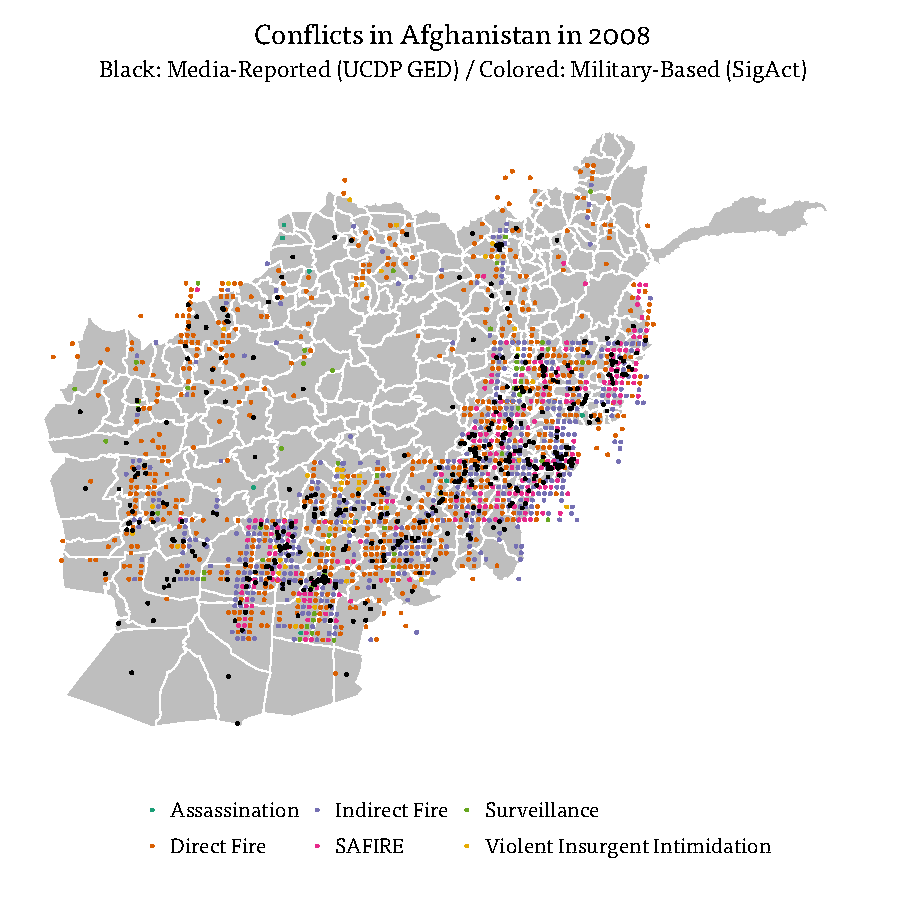
\includegraphics[width=.85\linewidth]{afg_map.pdf}
\end{figure}
\end{adjustwidth}

\columnbreak

\begin{minipage}{.65\linewidth}

\begin{table}[H] 
\small 
\vspace{-.5in}
\hspace{.6in}
\begin{tabular}{@{\extracolsep{5pt}}lccccccccc} 
\toprule
 & \multicolumn{3}{c}{\textbf{Media-Reported Data}}
 & \multicolumn{3}{c}{\textbf{Military-Based Data}}
 & \multicolumn{3}{c}{\textbf{Report Bias ($:=\mbox{Military}-\mbox{Media}$)}} \\ 
\cline{2-4} \cline{5-7} \cline{8-10}
\\[-1.8ex] & $\one(\mbox{Conflict}>0)$ & \multicolumn{2}{c}{Conflict Count} & $\one(\mbox{Conflict}>0)$ & \multicolumn{2}{c}{Conflict Count} & $\one(\mbox{Bias}>0)$ & \multicolumn{2}{c}{Report Bias} \\ 
 & Logit & ZINB & ZIP & Logit & ZINB & ZIP & Logit & ZINB & ZIP  \\ 
\midrule
 Cell Phone & 0.971$^{**}$ & 0.696$^{**}$ & 0.548$^{***}$ & 0.071 & 0.373 & 0.430$^{***}$ & 0.235 & 0.256 & 0.373$^{***}$ \\ 
\;\;\;Coverage  & (0.451) & (0.304) & (0.204) & (0.428) & (0.244) & (0.100) & (0.435) & (0.255) & (0.120) \\ 
  & & & & & & & & & \\[-1.8ex]
 Log Population & 0.347$^{**}$ & 0.774$^{***}$ & 0.786$^{***}$ & 0.398$^{***}$ & 0.477$^{***}$ & 0.549$^{***}$ & 0.376$^{**}$ & 0.400$^{***}$ & 0.444$^{***}$ \\ 
\;\;\;Density  & (0.160) & (0.115) & (0.066) & (0.148) & (0.099) & (0.038) & (0.151) & (0.110) & (0.045) \\ 
  & & & & & & & & & \\[-1.8ex] 
 Log Distance & 0.406$^{**}$ & 0.383$^{***}$ & 0.370$^{***}$ & $-$0.080 & 0.291$^{***}$ & 0.350$^{***}$ & $-$0.060 & 0.237$^{**}$ & 0.334$^{***}$ \\ 
\;\;\;Nearst City  & (0.177) & (0.125) & (0.081) & (0.160) & (0.102) & (0.043) & (0.163) & (0.110) & (0.053) \\ 
  & & & & & & & & & \\[-1.8ex] 
Spatial Lag & 0.163$^{***}$ & 0.041$^{***}$ & 0.038$^{***}$ & 0.078$^{***}$ & 0.016$^{***}$ & 0.013$^{***}$ & 0.079$^{***}$ & 0.014$^{***}$ & 0.012$^{***}$ \\ 
\;\;\;of Conflict & (0.024) & (0.007) & (0.004) & (0.010) & (0.002) & (0.0005) & (0.010) & (0.002) & (0.001) \\ 
  & & & & & & & & & \\[-1.8ex] 
 Constant & $-$7.524$^{***}$ & $-$10.388$^{***}$ & $-$10.232$^{***}$ & $-$5.275$^{***}$ & $-$5.629$^{***}$ & $-$6.355$^{***}$ & $-$5.428$^{***}$ & $-$4.734$^{***}$ & $-$5.334$^{***}$ \\ 
  & (1.992) & (1.580) & (1.018) & (1.770) & (1.248) & (0.528) & (1.818) & (1.354) & (0.623) \\ 
  & & & & & & & & & \\[-1.8ex] 
\hline \\[-1.8ex] 
Observations & 398 & 398 & 398 & 398 & 398 & 398 & 398 & 398 & 398 \\ 
Log Likelihood & $-$188.532 & $-$356.073 & $-$373.607 & $-$210.449 & $-$648.544 & $-$894.476 & $-$203.118 & $-$567.883 & $-$751.396 \\ 
\bottomrule
\end{tabular} 
\end{table} 

\end{minipage}

\section{Models: Binary Response and Event Count}

\begin{adjustwidth}{0.1in}{0.1in}
\setlength\abovedisplayskip{30pt} % spacing above equations
\setlength\abovedisplayshortskip{15pt} % spacing immediately above equations
\setlength\belowdisplayskip{0pt} % spacing below equations
\setlength\belowdisplayshortskip{0pt} % spacing immediately below equations
For district $i$,
\begin{align*}
\mathrm{Conflict}_i&=\alpha+\beta\cdot\mathrm{CellCoverage}_i+\gamma\cdot\log(\mathrm{Population})_i\\
&+\delta\cdot\log(\mathrm{DistNearCity})_i+\theta\cdot\mathrm{SpatialLag}_i+\varepsilon_i
\end{align*}

\vspace{.3in}
Possibly fake zeros, also extend to zero-inflated models
\begin{align*}
P(\mathrm{Conflict}_i=y_i)=
\left\{
\begin{array}{ll}
\pi_i+(1-\pi_i)f_Y(0|\lambda_i) & \mbox{if } y_i=0, \\
(1-\pi_i)f_Y(y_i|\lambda_i) & \mbox{if } y_i>0.
\end{array}
\right.
\end{align*}
\end{adjustwidth}



\section{Finding: Corr(Rep Bias, Cell Cov) is Low}


\begin{adjustwidth}{0.1in}{0.1in}
\begin{figure}
\centering
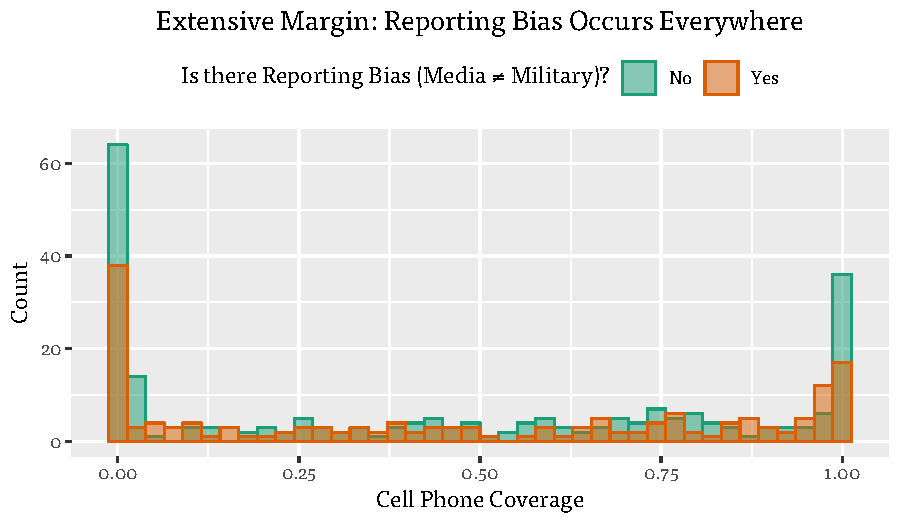
\includegraphics[width=\linewidth]{extensive.pdf}
\end{figure}
\end{adjustwidth}


\begin{adjustwidth}{0.1in}{0.1in}
\begin{figure}
\vspace{-1.6in} 
\hspace{6.8in}
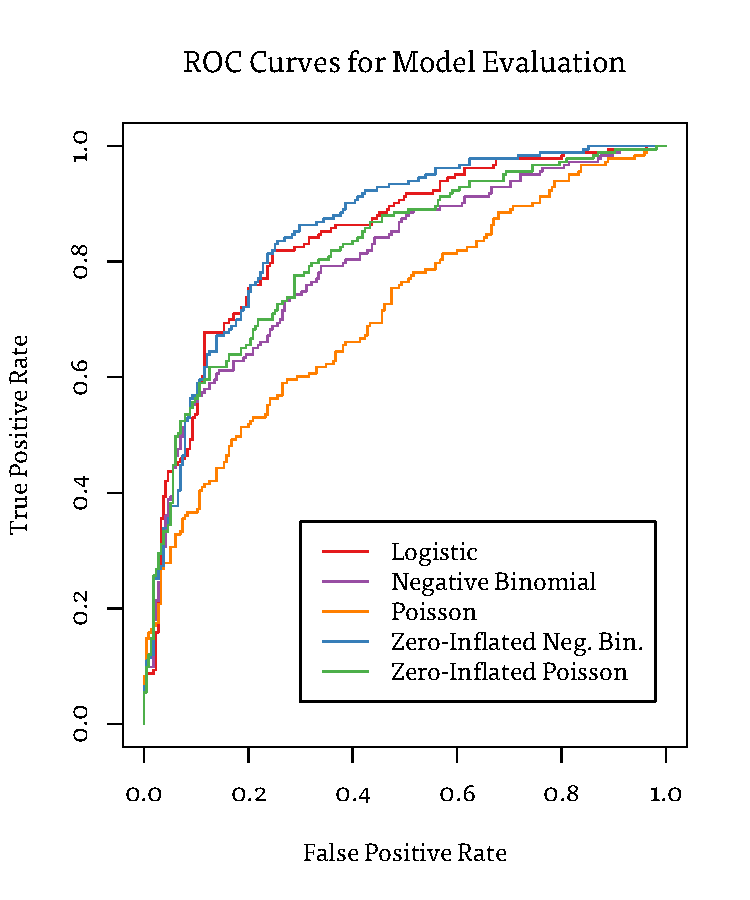
\includegraphics[width=.55\linewidth]{roc.pdf}
\end{figure}
\end{adjustwidth}


\vspace{-1.8in}
\begin{center}
\small
Predicted Probability of Conflict Being Reported Based on Cell Phone Coverage
\end{center}
\vspace{-.5in}
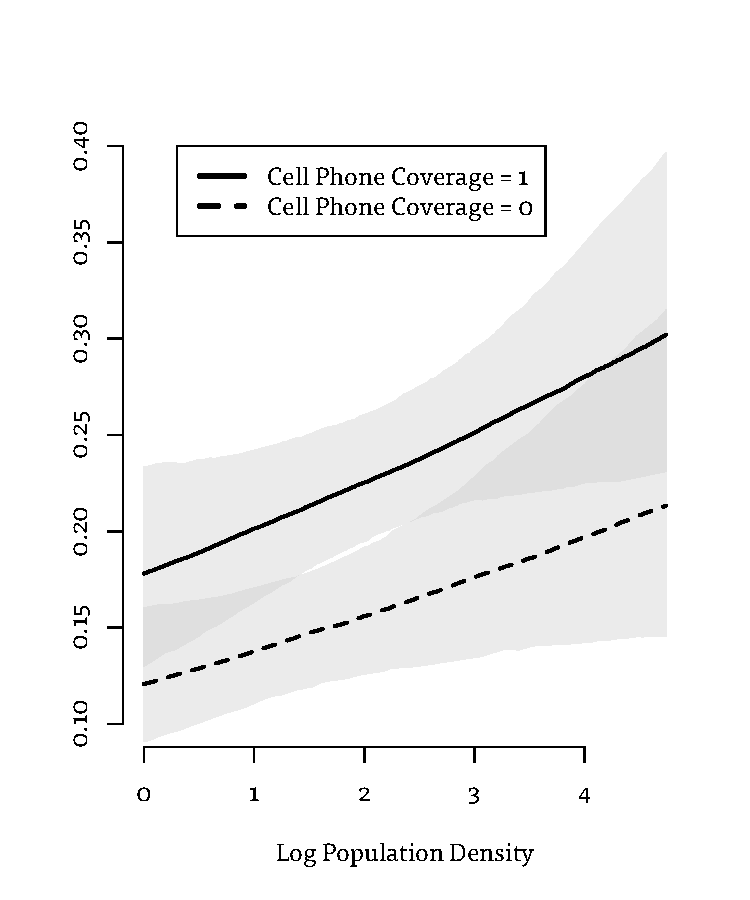
\includegraphics[width=.5\linewidth]{popu.pdf}
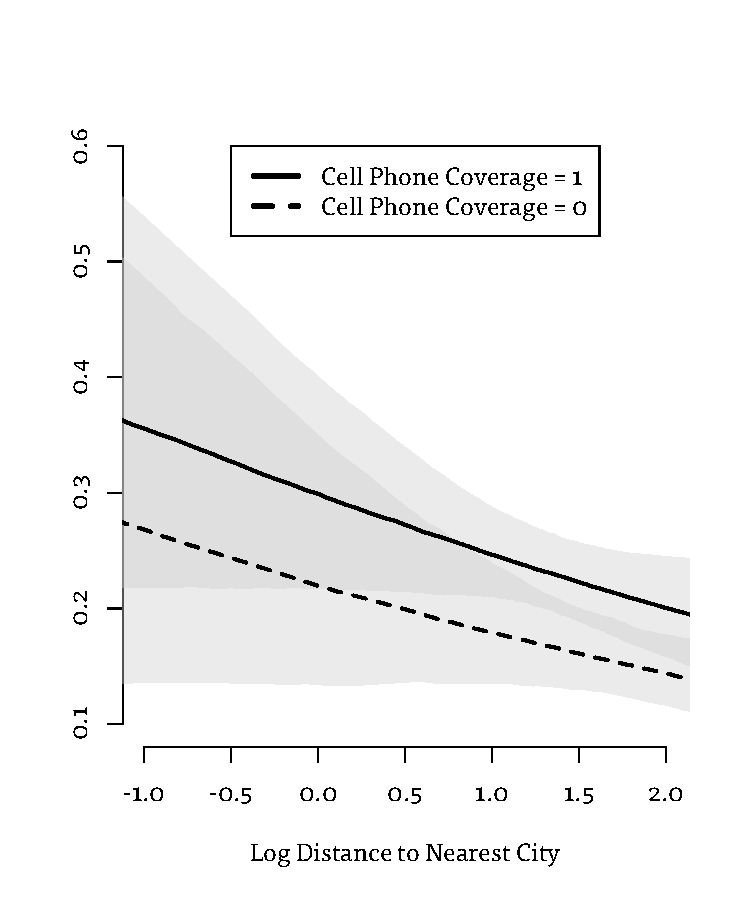
\includegraphics[width=.5\linewidth]{dist.pdf}


% \section{Next Steps}

% \begin{adjustwidth}{0.1in}{0.1in}

% Aliquam sed faucibus risus, quis efficitur erat. Vestibulum semper
% mauris quis tempus eleifend. Aliquam sagittis dictum ipsum, quis viverra
% ligula eleifend ut. Curabitur sagittis vitae arcu eget faucibus. In non
% elementum felis. 

% \end{adjustwidth}

% \section{Conclusion}

% \begin{adjustwidth}{0.1in}{0.1in}

% Duis \texttt{et} aliquam nunc. Nunc pulvinar sapien nunc, vel
% pretium nisi efficitur in. \texttt{Fusce} fringilla maximus leo et maximus. Fusce
% at ligula laoreet, iaculis mi at, auctor odio. Praesent sed elementum
% justo. Aenean consectetur risus rhoncus tincidunt efficitur. Praesent
% dictum mauris at diam maximus maximus.
% \end{adjustwidth}

\begin{figure}
\centering
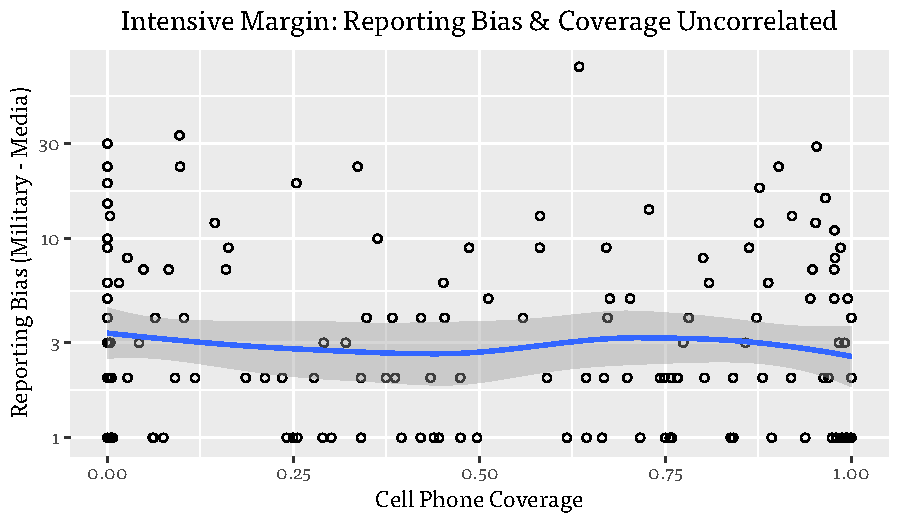
\includegraphics[width=\linewidth]{intensive.pdf}
\end{figure}


% \bibliographystyle{bib/econ_aer}
% \bibliography{bib/All_Papers}


\end{adjmulticols*}
%------------------ Body End ---------------------%
%end the poster

\end{document}

